\documentclass{article}
\usepackage{graphicx} % Extended graphics inclusions
\usepackage{float}
\usepackage{url} % For \url{}
\usepackage{../config/atxy} % For front cover
\usepackage{amsfonts} % Needed for some fonts
\usepackage[usenames]{color} % Needed for colored R input/output
\usepackage{pdfcolmk} % Correct some problems with the color stack


\title{Importing sequences from ACNUC databases}

\author{Charif, D. \and Lobry, J.R.}

\usepackage{Sweave}
\begin{document}
%
% To change the R input/output style:
%
\definecolor{Soutput}{rgb}{0,0,0.56}
\definecolor{Sinput}{rgb}{0.56,0,0}
\DefineVerbatimEnvironment{Sinput}{Verbatim}
{formatcom={\color{Sinput}},fontsize=\footnotesize, baselinestretch=0.75}
\DefineVerbatimEnvironment{Soutput}{Verbatim}
{formatcom={\color{Soutput}},fontsize=\footnotesize, baselinestretch=0.75}
%
% This removes the extra spacing after code and output chunks in Sweave,
% but keeps the spacing around the whole block.
%
\fvset{listparameters={\setlength{\topsep}{0pt}}}
\renewenvironment{Schunk}{\vspace{\topsep}}{\vspace{\topsep}}
%
% Rlogo
%
\newcommand{\Rlogo}{\protect
\includegraphics[height=1.8ex,keepaspectratio]{../figs/Rlogo.pdf}}
%
% Shortcut for seqinR:
%
\newcommand{\seqinr}{\texttt{seqin\bf{R}}}
\newcommand{\Seqinr}{\texttt{Seqin\bf{R}}}
\fvset{fontsize= \scriptsize}
%
% R output options and libraries to be loaded.
%
%
%  Sweave Options
%
% Put all figures in the fig folder and start the name with current file name.
% Do not produce EPS files
%


\maketitle
\tableofcontents
% BEGIN - DO NOT REMOVE THIS LINE

\section*{Introduction}

As a rule of thumb, after compression one nucleotide needs one octet
of disk space storage (because you need also the annotations corresponding
to the sequences), so that most likely you won't have enough space on
your computer to work with a local copy of a complete DNA database.
The idea is to import under \Rlogo{}~only the subset of sequences you are
interested in. This is done in three steps:
\begin{enumerate}
\item Choose the bank you want to work with.
\item Select the sequences you are interested in.
\item Retrieve sequences from server into your workspace.
\end{enumerate}
We now give a full example of those three steps under the ACNUC system
\cite{GautierC1982a, GautierC1982b, acnuc1984, acnuc1985, acnuc1985b}.

\section{Choose a bank}

Select the database from which you want to extract sequences with the \texttt{choosebank()} function.
This function initiates a remote access to an ACNUC database. Called without arguments,
\texttt{choosebank()} returns the list of available databases:


\begin{Schunk}
\begin{Sinput}
 choosebank()
\end{Sinput}
\begin{Soutput}
 [1] "genbank"        "embl"           "emblwgs"        "swissprot"     
 [5] "ensembl"        "refseq"         "refseqViruses"  "nrsub"         
 [9] "hobacnucl"      "hobacprot"      "hovergendna"    "hovergen"      
[13] "hogenom5"       "hogenom5dna"    "hogenom"        "hogenomdna"    
[17] "hogennucl"      "hogenprot"      "hoverclnu"      "hoverclpr"     
[21] "homolens3"      "homolens3dna"   "homolens"       "homolensdna"   
[25] "greviews"       "polymorphix"    "emglib"         "HAMAPnucl"     
[29] "HAMAPprot"      "taxobacgen"     "apis"           "anopheles"     
[33] "caenorhabditis" "ciona_savignyi" "danio"          "drosophila"    
[37] "felis"          "gallus"         "human"          "mouse"         
[41] "saccharomyces"  "tetraodon"      "xenopus"       
\end{Soutput}
\end{Schunk}
 

Biological sequence databases are fast moving targets, and for publication purposes it is
recommended to specify on which release you were working on when you made the job.
To get more informations about available databases on the server, just set 
the \texttt{infobank} parameter to \texttt{TRUE}. For
instance, here is the result for the three first databases on the default server 
at the compilation time (\today) of this document:

\begin{Schunk}
\begin{Sinput}
 choosebank(infobank = TRUE)[1:3, ]
\end{Sinput}
\begin{Soutput}
     bank status
1 genbank     on
2    embl     on
3 emblwgs     on
                                                                  info
1        GenBank Rel. 174 (15 October 2009) Last Updated: Nov  5, 2009
2 EMBL Library Release 101 (September 2009) Last Updated: Nov  5, 2009
3    EMBL Whole Genome Shotgun sequences Release 101  (September 2009)
\end{Soutput}
\end{Schunk}


Note that there is a \texttt{status} column because a database could be unavailable
for a while during updates. If you try call \texttt{choosebank(bank = "bankname")} 
when the bank called \texttt{bankname} is off from server, you will get an explicit 
error message stating that this bank is temporarily unavailable, for instance:

\begin{Schunk}
\begin{Sinput}
 res <- try(choosebank("off"))
 cat(res)
\end{Sinput}
\begin{Soutput}
Error in acnucopen(bank, socket) : 
  Database with name -->off<-- is currently off for maintenance, please try again later.
\end{Soutput}
\end{Schunk}

Some special purpose databases are not listed by default. These are \textit{tagged} databases
that are only listed if you provide an explicit \texttt{tagbank} argument to the \texttt{choosebank()}
function. Of special interest for teaching purposes is the \texttt{TP} tag, an acronym for
\textit{Travaux Pratiques} which means "practicals", and corresponds to \emph{frozen}
databases so that you can set up a practical whose results are stable from year to year. Currently
available frozen databases at the default server are:

\begin{Schunk}
\begin{Sinput}
 choosebank(tagbank = "TP", infobank = TRUE)
\end{Sinput}
\begin{Soutput}
         bank status                                           info
1      emblTP     on                            frozen EMBL release
2 swissprotTP     on                       frozen SwissProt release
3 hoverprotTP     on    frozen Hovergen release - protein sequences
4 hovernuclTP     on frozen Hovergen release - nucleotide sequences
5     trypano     on                        frozen trypano database
\end{Soutput}
\end{Schunk}


Now, if you want to work with a given database, say GenBank, just call \texttt{choosebank()}
with \texttt{"genbank"} as its first argument, the result is saved in the variable
\texttt{banknameSocket} in the workspace:

\begin{Schunk}
\begin{Sinput}
 choosebank("genbank")
 str(banknameSocket)
\end{Sinput}
\begin{Soutput}
List of 9
 $ socket  :Classes 'sockconn', 'connection'  atomic [1:1] 5
  .. ..- attr(*, "conn_id")=<externalptr> 
 $ bankname: chr "genbank"
 $ banktype: chr "GENBANK"
 $ totseqs : num 1.19e+08
 $ totspecs: num 686783
 $ totkeys : num 15791073
 $ release : chr "         GenBank Rel. 174 (15 October 2009) Last Updated: Nov  5, 2009"
 $ status  :Class 'AsIs'  chr "on"
 $ details : chr [1:4] "             ****     ACNUC Data Base Content      ****                         " "         GenBank Rel. 174 (15 October 2009) Last Updated: Nov  5, 2009" "108,943,317,873 bases; 111,355,981 sequences; 7,239,424 subseqs; 573,990 refers." "Software by M. Gouy, Lab. Biometrie et Biologie Evolutive, Universite Lyon I "
\end{Soutput}
\begin{Sinput}
 closebank()
\end{Sinput}
\end{Schunk}

The components of \texttt{banknameSocket} means that in the database
called \texttt{genbank} at the compilation time
of this document there were 
\texttt{118,595,406}
sequences from
\texttt{686,783}
species and a total of
\texttt{15,791,073}
keywords. The status of the bank was
\texttt{on}, 
and the release information was
\texttt{         GenBank Rel. 174 (15 October 2009) Last Updated: Nov  5, 2009}.
For specialized databases, some relevant informations are also given in the
\texttt{details} component, for instance:

\begin{Schunk}
\begin{Sinput}
 choosebank("taxobacgen")
 cat(banknameSocket$details, sep = "\n")
\end{Sinput}
\begin{Soutput}
               ****     ACNUC Data Base Content      ****
                 TaxoBacGen Rel. 7 (September 2005)
1,151,149,763 bases; 254,335 sequences; 847,767 subseqs; 63,879 refers.
	Data compiled from GenBank by Gregory Devulder 
        Laboratoire de Biometrie & Biologie Evolutive, Univ Lyon I
------------------------------
This database is a taxonomic genomic database. 
It results from an expertise crossing the data nomenclature database DSMZ
[http://www.dsmz.de/species/bacteria.htm Deutsche Sammlung von
Mikroorganismen und Zellkulturen GmbH, Braunschweig, Germany]
and GenBank. 
- Only contains sequences described under species present in 
Bacterial Nomenclature Up-to-date.
- Names of species and genus validly published according to the
Bacteriological Code (names with standing in nomenclature) is 
added in field "DEFINITION".
- A keyword "type strain" is added in field "FEATURES/source/strain" in
GenBank format definition to easyly identify Type Strain.
Taxobacgen is a genomic database designed for studies based on a strict
respect of up-to-date nomenclature and taxonomy.
\end{Soutput}
\begin{Sinput}
 closebank()
\end{Sinput}
\end{Schunk}

As from \seqinr~1.0-3, the result of the \texttt{choosebank()} function is automatically
stored in a global variable named \texttt{banknameSocket}, so that if no socket argument
is given to the \texttt{query()} function, the last opened database will be used by default
for your requests.
This is just a matter of convenience so that you don't have to explicitly specify the details of the
socket connection when working with the last opened database. You have, however,
full control of the process since \texttt{choosebank()} returns (invisibly) all the
required details. There is no trouble to open \emph{simultaneously} many databases.
You are just limited by the number of simultaneous connections your build of \Rlogo{}~is
allowed\footnote{
As from \Rlogo{}~2.4.0 he maximum number of open connections has been increased from
50 to 128. Note also that 
there is a very convenient function called \texttt{closeAllConnections()} in the \Rlogo{}~base package if
you want to close all open connections at once.}.

For advanced users who may wish to access to more than one database at time, a good advice
is to close them with the function \texttt{closebank()} as soon as possible so that the maximum
number of simultaneous connections is never reached. In the example below, we want to
display the number of taxa (\textit{i.e.} the number of nodes) in the species taxonomy associated
with each available database (including frozen databases). For this, we loop over available databases and 
close them as soon as the information has been retrieved.

\begin{Schunk}
\begin{Sinput}
 banks <- c(choosebank(), choosebank(tagbank = "TP"))
 nbanks <- length(banks)
 ntaxa <- numeric(nbanks)
 for (i in seq_len(nbanks)) {
     bkopenres <- try(choosebank(banks[i]))
     if (inherits(bkopenres, "try-error")) {
         ntaxa[i] <- NA
     }
     else {
         ntaxa[i] <- as.numeric(banknameSocket$totspecs)
         closebank()
     }
 }
 names(ntaxa) <- banks
\end{Sinput}
\end{Schunk}
\begin{Schunk}
\begin{Sinput}
 dotchart(log10(ntaxa[order(ntaxa)]), pch = 19, main = "Number of taxa in available databases", 
     xlab = "Log10(number of taxa)")
\end{Sinput}
\end{Schunk}
\includegraphics{../figs/getseqacnuc-plottaxaperbank}

\section{Make your query}

For this section, set up the default bank to GenBank, so that you don't have 
to provide the sockets details for the \texttt{query()} function:

\begin{Schunk}
\begin{Sinput}
 choosebank("genbank")
\end{Sinput}
\end{Schunk}

Then, you have to say what you want, that is to compose a query
to select the subset of sequences you are interested in. The way to do this is
documented under \texttt{?query}, we just give here a simple example
(more details are given in chapter \ref{querylang} page \pageref{querylang}). 
In the query below, we want to select all the coding sequences 
(\texttt{t=cds}) from cat (\texttt{AND sp=felis catus}) that are not 
(\texttt{AND NOT}) partial sequences (\texttt{k=partial}). 
We want the result to be stored in an object called \texttt{completeCatsCDS}.

\marginpar{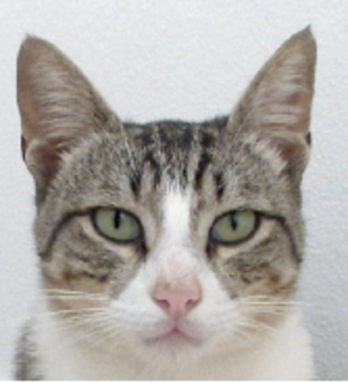
\includegraphics[width=\marginparwidth]{../figs/Feliscatus}\\
\tiny{\textit{Felis catus}. Source: wikipedia}}

\begin{Schunk}
\begin{Sinput}
 query("completeCatsCDS", "sp=felis catus AND t=cds AND NOT k=partial")
\end{Sinput}
\end{Schunk}

Now, there is in the workspace an object called \texttt{completeCatsCDS}, which
does not contain the sequences themselves but the \emph{sequence names} (and various relevant informations
such as the genetic code and the frame) that fit 
the query. They are stored in the \texttt{req} component of the object,
let's see the name of the first ten of them:

\begin{Schunk}
\begin{Sinput}
 getName(completeCatsCDS$req[1:10])
\end{Sinput}
\begin{Soutput}
 [1] "AB000483.PE1"    "AB000484.PE1"    "AB000485.PE1"    "AB003366"       
 [5] "AB003367"        "AB004237"        "AB004238"        "AB009279.PE1"   
 [9] "AB009280.PE1"    "AB010872.UGT1A1"
\end{Soutput}
\end{Schunk}

The first sequence that fit our request is \texttt{AB000483.PE1},
the second one is \texttt{AB000484.PE1}, and so on. Note that
the sequence name may have an extension, this corresponds to \emph{subsequences},
a specificity of the ACNUC system that allows to handle easily a
subsequence with a biological meaning, typically a gene. The list of available subsequences
in a given database is given by the function \texttt{getType()}, for example the list
of available subsequences in GenBank is given in table \ref{genbank}.

%
% Besoin d'edition manuelle du fichier genbank.tex pour virer les caracteres sp�ciaux Latex, ici "_"
%
% latex table generated in R 2.1.0 by xtable 1.2-5 package
% Wed Jul 20 12:00:16 2005
\begin{table}[ht]
\begin{center}
\begin{tabular}{rll}
\hline
 & Type & Description \\
\hline
1 &      CDS &              .PE protein coding region \\
2 &    LOCUS &                 sequenced DNA fragment \\
3 & MISC\_RNA & .RN other structural RNA coding region \\
4 &     RRNA &               .RR mature ribosomal RNA \\
5 &    SCRNA &              .SC small cytoplasmic RNA \\
6 &    SNRNA &                  .SN small nuclear RNA \\
7 &     TRNA &                .TR mature transfer RNA \\
\hline
\end{tabular}
\caption{Available subsequences in genbank}
\label{genbank}
\end{center}
\end{table}



The component \texttt{call} of \texttt{completeCatsCDS} keeps automatically a 
trace of the way you have selected the sequences: 

\begin{Schunk}
\begin{Sinput}
 completeCatsCDS$call
\end{Sinput}
\begin{Soutput}
query(listname = "completeCatsCDS", query = "sp=felis catus AND t=cds AND NOT k=partial")
\end{Soutput}
\end{Schunk}

At this stage you can quit your \Rlogo{} 
session saving the workspace image. The next time an \Rlogo{}~session is opened with the 
workspace image restored, there will be an object called \texttt{completeCatsCDS}, and 
looking into its \texttt{call} component will tell you that it contains the names 
of complete coding sequences from \textit{Felis catus}.

In practice, queries for sequences are rarely done in one step and are more likely
to be the result of an iterative, progressively refining, process. An important point
is that a list of sequences can be re-used. For instance, we can re-use \texttt{completeCatsCDS}
to get only the list of sequences that were published in 2004:

\begin{Schunk}
\begin{Sinput}
 query("ccc2004", "completeCatsCDS AND y=2004")
 length(ccc2004$req)
\end{Sinput}
\begin{Soutput}
[1] 60
\end{Soutput}
\begin{Sinput}
 ccc2004$nelem
\end{Sinput}
\begin{Soutput}
[1] 60
\end{Soutput}
\end{Schunk}

Hence, there were 60 complete coding sequences published in 2004 for
\textit{Felis catus} in GenBank.

As from release 1.0-3 of the \seqinr{} package, there is new parameter \texttt{virtual}
which allows to disable the automatic retrieval of information for all list elements. This is interesting for list
with many elements, for instance :

\begin{Schunk}
\begin{Sinput}
 query("allcds", "t=cds", virtual = TRUE)
 allcds$nelem
\end{Sinput}
\begin{Soutput}
[1] 7992598
\end{Soutput}
\end{Schunk}

There are therefore \texttt{7,992,598} coding
sequences in this version of GenBank\footnote{
which is stored in the \texttt{release} component of the object \texttt{banknameSocket}
and current value is today (\today): \texttt{banknameSocket\$release = 
         GenBank Rel. 174 (15 October 2009) Last Updated: Nov  5, 2009}.
}. 
It would be long to get all the informations for the elements
of this list, so we have set the parameter \texttt{virtual} to \texttt{TRUE} and the \texttt{req}
component of the list has not been documented:

\begin{Schunk}
\begin{Sinput}
 allcds$req
\end{Sinput}
\begin{Soutput}
[1] NA
\end{Soutput}
\end{Schunk}

However, the list can still be re-used\footnote{
of course, as long as the socket connection with the server has not been lost: virtual lists details are only
known by the server.}, 
for instance we may extract from this list all the sequences
from, say, \textit{Mycoplasma genitalium}:

\begin{Schunk}
\begin{Sinput}
 query("small", "allcds AND sp=mycoplasma genitalium", virtual = TRUE)
 small$nelem
\end{Sinput}
\begin{Soutput}
[1] 979
\end{Soutput}
\end{Schunk}

There are then \texttt{979} elements in
the list \texttt{small}, so that we can safely repeat the previous query without asking for a
virtual list:

\begin{Schunk}
\begin{Sinput}
 query("small", "allcds et sp=mycoplasma genitalium")
 getName(small$req[1:10])
\end{Sinput}
\begin{Soutput}
 [1] "AY191424" "AY386807" "AY386808" "AY386809" "AY386810" "AY386811"
 [7] "AY386812" "AY386813" "AY386814" "AY386815"
\end{Soutput}
\end{Schunk}

Here are some illustrations of using virtual list to answer simple questions about the
current GenBank release.

\begin{description}
\item[\textbf{Man.}] How many sequences are available for our species?
\begin{Schunk}
\begin{Sinput}
 query("man", "sp=homo sapiens", virtual = T)
 man$nelem
\end{Sinput}
\begin{Soutput}
[1] 13042724
\end{Soutput}
\end{Schunk}
There are \texttt{13,042,724} sequences from \textit{Homo sapiens}.

\item[\textbf{Sex.}] How many sequences are annotated with a keyword starting by sex?
\begin{Schunk}
\begin{Sinput}
 query("sex", "k=sex@", virtual = T)
 sex$nelem
\end{Sinput}
\begin{Soutput}
[1] 1465
\end{Soutput}
\end{Schunk}
There are \texttt{1,465} such sequences.

\item[\textbf{tRNA.}] How many complete tRNA sequences are available?
\begin{Schunk}
\begin{Sinput}
 query("trna", "t=trna AND NOT k=partial", virtual = T)
 trna$nelem
\end{Sinput}
\begin{Soutput}
[1] 413347
\end{Soutput}
\end{Schunk}
There are \texttt{413,347} complete tRNA sequences.

\item[\textbf{Nature vs. Science.}] In which journal were the more sequences published?
\begin{Schunk}
\begin{Sinput}
 query("nature", "j=nature", virtual = T)
 nature$nelem
\end{Sinput}
\begin{Soutput}
[1] 1992670
\end{Soutput}
\begin{Sinput}
 query("science", "j=science", virtual = T)
 science$nelem
\end{Sinput}
\begin{Soutput}
[1] 1530942
\end{Soutput}
\end{Schunk}
There are \texttt{1,992,670} sequences published
in \textit{Nature} and
\texttt{1,530,942} sequences published in
\textit{Science}, so that the winner is 
\textit{Nature}.

%
% \item[TriTryp] quand la ref de Science/309/404 sera dans genbank
%

\item[\textbf{Smith.}] How many sequences have Smith (last name) as author?
\begin{Schunk}
\begin{Sinput}
 query("smith", "au=smith", virtual = T)
 smith$nelem
\end{Sinput}
\begin{Soutput}
[1] 4809459
\end{Soutput}
\end{Schunk}
There are \texttt{4,809,459} such sequences.

\item[\textbf{YK2.}] How many sequences were published after year 2000 (included)?
\begin{Schunk}
\begin{Sinput}
 query("yk2", "y>2000", virtual = T)
 yk2$nelem
\end{Sinput}
\begin{Soutput}
[1] 99752843
\end{Soutput}
\end{Schunk}
There are \texttt{99,752,843} sequences published after year 2000.

\item[\textbf{Organelle contest.}] Do we have more sequences from chloroplast genomes or from mitochondion genomes?
\begin{Schunk}
\begin{Sinput}
 query("chloro", "o=chloroplast", virtual = T)
 chloro$nelem
\end{Sinput}
\begin{Soutput}
[1] 255832
\end{Soutput}
\begin{Sinput}
 query("mito", "o=mitochondrion", virtual = T)
 mito$nelem
\end{Sinput}
\begin{Soutput}
[1] 815726
\end{Soutput}
\end{Schunk}
There are \texttt{255,832} sequences from
chloroplast genomes and
\texttt{815,726} sequences from mitochondrion
genomes, so that the winner is 
mitochondrion.


\end{description}

\begin{Schunk}
\begin{Sinput}
 closebank()
\end{Sinput}
\end{Schunk}


\section{Extract sequences of interest}

\subsection{Introduction}

There are two functions to get the sequences. The first one, 
\texttt{getSequence()}, uses regular socket connections, the
second one, \texttt{extractseqs()}, uses zlib compressed sockets,
which is faster but the function is experimental (details in
chapter \ref{extractseqs} page \pageref{extractseqs}).

\subsection{Extacting sequences with \texttt{getSequence()}}


For this section we set up the bank to \texttt{emblTP} which is a frozen
subset of EMBL database to allow for the reproducibility of results.

\begin{Schunk}
\begin{Sinput}
 choosebank("emblTP")
\end{Sinput}
\end{Schunk}

We suppose that the sequences we are interested in are all the complete
coding sequences from \textit{Felis catus} :

\begin{Schunk}
\begin{Sinput}
 query("completeCatsCDS", "sp=felis catus AND t=cds AND NOT k=partial")
 (nseq <- completeCatsCDS$nelem)
\end{Sinput}
\begin{Soutput}
[1] 257
\end{Soutput}
\end{Schunk}

Thus, there were 257 complete
CDS from \textit{Felis catus} in this release of EMBL.


The sequences are obtained with the function \texttt{getSequence()}.
For example, the first 50 nucleotides of the first sequence of our request are:

\begin{Schunk}
\begin{Sinput}
 myseq <- getSequence(completeCatsCDS$req[[1]])
 myseq[1:50]
\end{Sinput}
\begin{Soutput}
 [1] "a" "t" "g" "a" "c" "c" "a" "a" "c" "a" "t" "t" "c" "g" "a" "a" "a" "a"
[19] "t" "c" "a" "c" "a" "c" "c" "c" "c" "c" "t" "t" "a" "c" "c" "a" "a" "a"
[37] "a" "t" "t" "a" "t" "t" "a" "a" "t" "c" "a" "c" "t" "c"
\end{Soutput}
\end{Schunk}
They can also be coerced as string of character with the function \texttt{c2s()}:
\begin{Schunk}
\begin{Sinput}
 c2s(myseq[1:50])
\end{Sinput}
\begin{Soutput}
[1] "atgaccaacattcgaaaatcacacccccttaccaaaattattaatcactc"
\end{Soutput}
\end{Schunk}

We can also use the argument \texttt{as.string} to retrive sequences
directly as strings:

\begin{Schunk}
\begin{Sinput}
 substr(getSequence(completeCatsCDS$req[[1]], as.string = TRUE), 
     1, 50)
\end{Sinput}
\begin{Soutput}
[1] "atgaccaacattcgaaaatcacacccccttaccaaaattattaatcactc"
\end{Soutput}
\end{Schunk}

Note that what is done by \texttt{getSequence()} is much more complex
than a simple substring extraction because subsequences of biological 
interest are not necessarily contiguous, nor on the same DNA strand,
nor even from the same entry. 

\subsection{Extracting sequences with trans-splicing}

Consider for
instance the following coding sequence from sequence \texttt{AE003734}:

\begin{Schunk}
\begin{Sinput}
 query("trs", "N=AE003734.PE35")
 annots <- getAnnot(trs$req[[1]])
 cat(annots, sep = "\n")
\end{Sinput}
\begin{Soutput}
FT   CDS             join(complement(153944..154157),complement(153727..153866),
FT                   complement(152185..153037),138523..138735,138795..138955)
FT                   /codon_start=1
FT                   /db_xref="FLYBASE:FBgn0002781"
FT                   /db_xref="GOA:Q86B86"
FT                   /db_xref="TrEMBL:Q86B86"
FT                   /note="mod(mdg4) gene product from transcript CG32491-RZ;
FT                   trans splicing"
FT                   /gene="mod(mdg4)"
FT                   /product="CG32491-PZ"
FT                   /locus_tag="CG32491"
FT                   /protein_id="AAO41581.1"
FT                   /translation="MADDEQFSLCWNNFNTNLSAGFHESLCRGDLVDVSLAAEGQIVKA
FT                   HRLVLSVCSPFFRKMFTQMPSNTHAIVFLNNVSHSALKDLIQFMYCGEVNVKQDALPAF
FT                   ISTAESLQIKGLTDNDPAPQPPQESSPPPAAPHVQQQQIPAQRVQRQQPRASARYKIET
FT                   VDDGLGDEKQSTTQIVIQTTAAPQATIVQQQQPQQAAQQIQSQQLQTGTTTTATLVSTN
FT                   KRSAQRSSLTPASSSAGVKRSKTSTSANVMDPLDSTTETGATTTAQLVPQQITVQTSVV
FT                   SAAEAKLHQQSPQQVRQEEAEYIDLPMELPTKSEPDYSEDHGDAAGDAEGTYVEDDTYG
FT                   DMRYDDSYFTENEDAGNQTAANTSGGGVTATTSKAVVKQQSQNYSESSFVDTSGDQGNT
FT                   EAQVTQHVRNCGPQMFLISRKGGTLLTINNFVYRSNLKFFGKSNNILYWECVQNRSVKC
FT                   RSRLKTIGDDLYVTNDVHNHMGDNKRIEAAKAAGMLIHKKLSSLTAADKIQGSWKMDTE
FT                   GNPDHLPKM"
\end{Soutput}
\end{Schunk}

To get the coding sequence manually you would have join 5 different pieces 
from \texttt{AE003734} and some of them are in the complementary strand. 
With \texttt{getSequence()} you don't have to think about this. Just make a
query with the sequence name:

\begin{Schunk}
\begin{Sinput}
 query("transspliced", "N=AE003734.PE35")
 length(transspliced$req)
\end{Sinput}
\begin{Soutput}
[1] 1
\end{Soutput}
\begin{Sinput}
 getName(transspliced$req[[1]])
\end{Sinput}
\begin{Soutput}
[1] "AE003734.PE35"
\end{Soutput}
\end{Schunk}

Ok, now there is in your workspace an object called \texttt{transspliced} which \texttt{req}
component is of length one (because you have asked for just one sequence) and the name of the
single element of the req component is AE003734.PE35 (because this
is the name of the sequence you wanted). Let see the first 50 base of this sequence:

\begin{Schunk}
\begin{Sinput}
 getSequence(transspliced$req[[1]])[1:50]
\end{Sinput}
\begin{Soutput}
 [1] "a" "t" "g" "g" "c" "g" "g" "a" "c" "g" "a" "c" "g" "a" "g" "c" "a" "a"
[19] "t" "t" "c" "a" "g" "c" "t" "t" "g" "t" "g" "c" "t" "g" "g" "a" "a" "c"
[37] "a" "a" "c" "t" "t" "c" "a" "a" "c" "a" "c" "g" "a" "a"
\end{Soutput}
\end{Schunk}

All the complex trans-splicing operations have been done here. You can check that there is no
in-frame stop codons\footnote{
Stop codons are represented by the character \texttt{*} when translated into protein.} 
with the \texttt{getTrans()} function to translate this coding sequence into protein:

\begin{Schunk}
\begin{Sinput}
 getTrans(transspliced$req[[1]])[1:50]
\end{Sinput}
\begin{Soutput}
 [1] "M" "A" "D" "D" "E" "Q" "F" "S" "L" "C" "W" "N" "N" "F" "N" "T" "N" "L"
[19] "S" "A" "G" "F" "H" "E" "S" "L" "C" "R" "G" "D" "L" "V" "D" "V" "S" "L"
[37] "A" "A" "E" "G" "Q" "I" "V" "K" "A" "H" "R" "L" "V" "L"
\end{Soutput}
\begin{Sinput}
 table(getTrans(transspliced$req[[1]]))
\end{Sinput}
\begin{Soutput}
 *  A  C  D  E  F  G  H  I  K  L  M  N  P  Q  R  S  T  V  W  Y 
 1 47  7 33 25 15 29 12 20 26 33 12 27 25 52 19 48 47 34  3 12 
\end{Soutput}
\end{Schunk}

In a more graphical way:

\begin{Schunk}
\begin{Sinput}
 aacount <- table(getTrans(transspliced$req[[1]]))
 aacount <- aacount[order(aacount)]
 names(aacount) <- aaa(names(aacount))
 dotchart(aacount, pch = 19, xlab = "Stop and amino-acid counts", 
     main = "There is only one stop codon in AE003734.PE35")
 abline(v = 1, lty = 2)
\end{Sinput}
\end{Schunk}
\includegraphics{../figs/getseqacnuc-transp4}

Note that the relevant variant of the genetic code was automatically set up during the translation
of the sequence into protein. This is because the \texttt{transspliced\$req[[1]]} object belongs to the 
\texttt{SeqAcnucWeb} class:

\begin{Schunk}
\begin{Sinput}
 class(transspliced$req[[1]])
\end{Sinput}
\begin{Soutput}
[1] "SeqAcnucWeb"
\end{Soutput}
\end{Schunk}

Therefore, when you are using the \texttt{getTrans()} function, you are automatically redirected
to the \texttt{getTrans.SeqAcnucWeb()} function which knows how to take into account the relevant frame
and genetic code for your coding sequence.

\subsection{Extracting sequences from many entries}

Consider the following CDS from \texttt{M19233}:

\begin{Schunk}
\begin{Sinput}
 query("multi", "AC=M19233 AND T=CDS")
 cat(getAnnot(multi$req[[1]]), sep = "\n")
\end{Sinput}
\begin{Soutput}
FT   CDS             join(M17883.1:988..1155,M17883.1:1504..1650,
FT                   M17883.1:2451..2648,M17883.1:3098..3328,625..758)
FT                   /codon_start=1
FT                   /db_xref="GOA:Q13763"
FT                   /db_xref="TrEMBL:Q13763"
FT                   /partial
FT                   /gene="AMY1A"
FT                   /product="alpha-amylase"
FT                   /protein_id="AAA57345.1"
FT                   /translation="MKLFWLLFTIGFCWAQYSSNTQQGRTSIVHLFEWRWVDIALECER
FT                   YLAPKGFGGVQVSPPNENVAIHNPFRPWWERYQPVSYKLCTRSGNEDEFRNMVTRCNNV
FT                   GVRIYVDAVINHMCGNAVSAGTSSTCGSYFNPGSRDFPAVPYSGWDFNDGKCKTGSGDI
FT                   ENYNDATQVRDCRLSGLLDPALGKDYVRSKIAEYMNHLIDIGVAGFRIDASKHMWPGDI
FT                   KAILDKLHNLNSNWFPEGSKPFIYQEVIDLGGEPIKSSDYFGNGRVTEFKYGAKLGTVI
FT                   RKWTGEKMSYL"
\end{Soutput}
\end{Schunk}

The CDS here is obtained by joining pieces from different entries,
but this is not a problem:

\begin{Schunk}
\begin{Sinput}
 getTrans(multi$req[[1]])
\end{Sinput}
\begin{Soutput}
  [1] "M" "K" "L" "F" "W" "L" "L" "F" "T" "I" "G" "F" "C" "W" "A" "Q" "Y" "S"
 [19] "S" "N" "T" "Q" "Q" "G" "R" "T" "S" "I" "V" "H" "L" "F" "E" "W" "R" "W"
 [37] "V" "D" "I" "A" "L" "E" "C" "E" "R" "Y" "L" "A" "P" "K" "G" "F" "G" "G"
 [55] "V" "Q" "V" "S" "P" "P" "N" "E" "N" "V" "A" "I" "H" "N" "P" "F" "R" "P"
 [73] "W" "W" "E" "R" "Y" "Q" "P" "V" "S" "Y" "K" "L" "C" "T" "R" "S" "G" "N"
 [91] "E" "D" "E" "F" "R" "N" "M" "V" "T" "R" "C" "N" "N" "V" "G" "V" "R" "I"
[109] "Y" "V" "D" "A" "V" "I" "N" "H" "M" "C" "G" "N" "A" "V" "S" "A" "G" "T"
[127] "S" "S" "T" "C" "G" "S" "Y" "F" "N" "P" "G" "S" "R" "D" "F" "P" "A" "V"
[145] "P" "Y" "S" "G" "W" "D" "F" "N" "D" "G" "K" "C" "K" "T" "G" "S" "G" "D"
[163] "I" "E" "N" "Y" "N" "D" "A" "T" "Q" "V" "R" "D" "C" "R" "L" "S" "G" "L"
[181] "L" "D" "P" "A" "L" "G" "K" "D" "Y" "V" "R" "S" "K" "I" "A" "E" "Y" "M"
[199] "N" "H" "L" "I" "D" "I" "G" "V" "A" "G" "F" "R" "I" "D" "A" "S" "K" "H"
[217] "M" "W" "P" "G" "D" "I" "K" "A" "I" "L" "D" "K" "L" "H" "N" "L" "N" "S"
[235] "N" "W" "F" "P" "E" "G" "S" "K" "P" "F" "I" "Y" "Q" "E" "V" "I" "D" "L"
[253] "G" "G" "E" "P" "I" "K" "S" "S" "D" "Y" "F" "G" "N" "G" "R" "V" "T" "E"
[271] "F" "K" "Y" "G" "A" "K" "L" "G" "T" "V" "I" "R" "K" "W" "T" "G" "E" "K"
[289] "M" "S" "Y" "L"
\end{Soutput}
\begin{Sinput}
 table(aaa(getTrans(multi$req[[1]])))
\end{Sinput}
\begin{Soutput}
Ala Arg Asn Asp Cys Gln Glu Gly His Ile Leu Lys Met Phe Pro Ser Thr Trp Tyr 
 15  16  19  17   8   7  14  28   6  17  18  16   6  15  14  21  12  10  14 
Val 
 19 
\end{Soutput}
\end{Schunk}

There is no stop codon here because the sequence is partial.


\begin{Schunk}
\begin{Sinput}
 closebank()
\end{Sinput}
\end{Schunk}


\section*{Session Informations}

\begin{scriptsize}

This part was compiled under the following \Rlogo{}~environment:

\begin{itemize}\raggedright
  \item R version 2.10.0 (2009-10-26), \verb|i386-apple-darwin8.11.1|
  \item Locale: \verb|fr_FR.UTF-8/fr_FR.UTF-8/fr_FR.UTF-8/C/C/C|
  \item Base packages: base, datasets, graphics, grDevices, grid,
    methods, stats, utils
  \item Other packages: ade4~1.4-13, ape~2.4, grImport~0.4-4,
    MASS~7.3-3, quadprog~1.4-11, seqinr~2.0-7, tseries~0.10-21,
    XML~2.6-0, xtable~1.5-5, zoo~1.5-8
  \item Loaded via a namespace (and not attached): gee~4.13-14,
    lattice~0.17-26, nlme~3.1-96, tools~2.10.0
\end{itemize}
There were two compilation steps:

\begin{itemize}
  \item \Rlogo{} compilation time was: Thu Nov  5 12:36:14 2009
  \item \LaTeX{} compilation time was: \today
\end{itemize}

\end{scriptsize}

% END - DO NOT REMOVE THIS LINE

%%%%%%%%%%%%  BIBLIOGRAPHY %%%%%%%%%%%%%%%%%
\clearpage
\addcontentsline{toc}{section}{References}
\bibliographystyle{plain}
\bibliography{../config/book}
\end{document}
